\documentclass{article}
\usepackage{multicol}
\usepackage[utf8]{inputenc}
\usepackage[T1]{fontenc}      
\usepackage[francais]{babel}
\usepackage{graphicx}
\usepackage{circuitikz}
\usepackage[squaren, Gray]{SIunits}
\usepackage{sistyle}
\usepackage[autolanguage]{numprint}
\usepackage{pgfplots}
\usepackage{geometry}
\usepackage{hyperref}
\usepackage{caption}
\usepackage{amsmath,amssymb,array}
\usepackage{url}
\usepackage{fancyhdr}
\usepackage{layout}
\usepackage[version=3]{mhchem}
\usepackage{array} 
\usepackage{tikz}
	\usetikzlibrary{arrows,shapes,positioning}


\newcommand{\reporttitle}{Analyse dynamique}     % Titre
\newcommand{\reportauthor}{Geoffroy \bsc{Jacquet} \\ Corentin \bsc{Joachim}\\ Léa \bsc{Paulus}} % Auteur
\newcommand{\reportsubject}{Rapport de projet en construction mécanique 1} % Sujet
\newcommand{\HRule}{\rule{\linewidth}{0.5mm}}
\newcommand{\copyrigh}{{\tiny \textregistered}}
\setlength{\parskip}{1ex} % Espace entre les paragraphes

\hypersetup{
    pdftitle={\reporttitle},%
     pdfauthor={\reportauthor},%
    pdfsubject={\reportsubject},%
    pdfkeywords={rapport} {vos} {mots} {clés}
}


\setlength{\headheight}{12pt}
\setlength{\headsep}{12pt}

\pagestyle{fancy}
\lhead{\leftmark{}}
\rhead{LMECA1210 - 2015 - gr11}
\cfoot{\thepage{}}
\begin{document}
\begin{titlepage}

\begin{center}

% Upper part of the page

\textsc{\Large Université Catholique de Louvain}\\[0.5cm]

\textsc{\LARGE Rapport de projet en construction mécanique 1}\\[0.2cm]
\textsc{\LARGE LMECA1210}\\[0.2cm]

% Title
\HRule \\[0.2cm]
{\huge \bfseries Analyse dynamique}\\
\HRule \\[0.2cm]

% Author and supervisor
\begin{center}
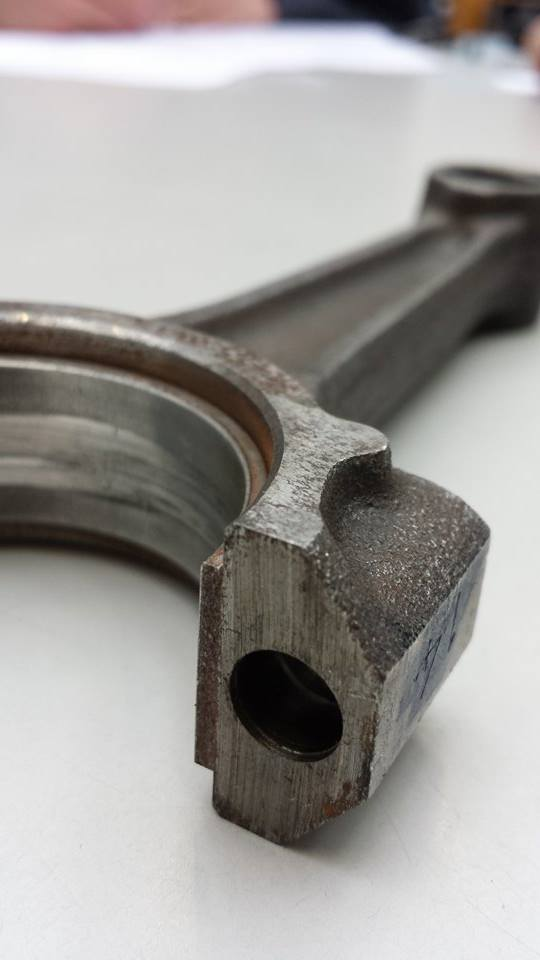
\includegraphics[trim=0cm 8cm 0cm 5cm, clip, width= 15 cm, height= 9.5 cm ]{Schema/bielle2.jpg}
\end{center}
\HRule \\[0 cm]


\begin{minipage}{0.4\textwidth}
\begin{flushleft} \large

\begin{tabular}{l l}

\emph{Auteurs:} & \\
 
Geoffroy & \bsc{Jacquet}\\ 
Corentin & \bsc{Joachim}\\ 
Léa & \bsc{Paulus}

\end{tabular}
\end{flushleft}
\end{minipage}
\begin{minipage}{0.4\textwidth}
\begin{flushright} \large
\emph{Cours:} \\
LMECA1210\\
\emph{Groupe:} \\
11\\
\emph{Professeur:} \\
Hervé \textsc{Jeanmart}
\end{flushright}
\end{minipage}
\vspace{0.3cm}
% Bottom of the page

\begin{minipage}{0.3\textwidth}
\begin{flushleft}

\includegraphics[height=2cm]{Schema/logo_UCL_NEW_janv2013.JPG}
\end{flushleft}
\end{minipage}
\begin{minipage}{0.3\textwidth}
\begin{center}
{\large FSA12BA}\\
{\large \today}
\end{center}
\end{minipage}
\begin{minipage}{0.3\textwidth}
\begin{flushright}

\includegraphics[height=1cm]{Schema/epl-logo.jpg}
\end{flushright}
\end{minipage}
\end{center}
\end{titlepage}
\tableofcontents
\section{Détermination des grandeurs géométriques du moteur}
\section{Évolution de le pression dans le cylindre}
\section{Effort sur la bielle en fonction de l'angle du vilebrequin}
\section{Justification de la forme en "I"}
La bielle étant contrainte à des efforts de traction et principalement de compression, pour un fonctionnement optimal dans un moteur à haute vitesse il faut que celle-ci soit à la fois élancée, légère tout en étant capable de résister aux sollicitations. La forme qui répond le mieux à l'ensemble de ces critères s'avère être la forme en I.
\section{Dimensionnement de la section de la bielle}
%don"t write in this one ! :)

\end{document}